
\documentclass[11pt]{article}

\usepackage[margin=1in]{geometry}
\usepackage[T1]{fontenc}
\usepackage[utf8]{inputenc}
\usepackage{lmodern}
\usepackage{setspace}
\usepackage{hyperref}
\usepackage{booktabs}
\usepackage{longtable}
\usepackage{array}
\usepackage{multirow}
\usepackage{graphicx}
\usepackage{float}
\usepackage{caption}
\usepackage{enumitem}
\usepackage{xcolor}
\usepackage{amsmath}
\usepackage{amssymb}

\hypersetup{
    colorlinks=true,
    linkcolor=blue,
    citecolor=blue,
    urlcolor=blue
}

\title{\textbf{Demonstrating Hallucination in Modern LLMs and Training a Response-Level Detector}\\
\vspace{0.75em}
\normalsize A Research Report on Benchmark Construction, Behavioral Analysis, and Hallucination Detection}
\author{Khanh Van}
\date{University of Texas at Austin\\Spring 2026}

\begin{document}
\maketitle
\onehalfspacing

\begin{abstract}
Hallucination remains one of the central reliability failures of modern large language models (LLMs): models can produce fluent, confident, and contextually plausible outputs that are factually unsupported or simply wrong. This report presents a two-part research project designed primarily as a \emph{demonstration study}. The first part constructs a lightweight benchmark to reveal hallucination behavior across four open and widely used models---TinyLlama, Phi-3 Mini, Mistral 7B Instruct, and LLaMA 3.1 8B Instruct---using a set of simple factual, hard factual, trap, and adversarial prompts. The benchmark is intentionally limited in topical depth and is not meant to estimate hallucination prevalence in specialized high-stakes domains such as law or medicine. Rather, it is designed to show that hallucination can still emerge even under relatively simple prompting conditions and that refusal behavior is a crucial safety mechanism.

The second part trains a machine learning detector on the collected response-level dataset to classify whether a generated answer is hallucinated. The detector is not a prompt-level predictor; instead, it operates \emph{after} generation, using features such as model confidence, refusal behavior, answer length, prompt category, and model identity. On the collected dataset, a Random Forest classifier achieved 93.3\% accuracy, 70.0\% precision, 87.5\% recall, an F1 score of 0.778, and ROC-AUC of 0.958. These results suggest that even a relatively simple tabular detector can capture meaningful behavioral signals associated with hallucination. The broader conclusion of the project is not that advanced models rarely hallucinate in general, but that simple benchmarks can demonstrate the phenomenon, and that stronger, domain-specific, evidence-grounded evaluation remains necessary for trustworthy deployment.
\end{abstract}
\newpage

\tableofcontents
\newpage

\section{Introduction}
Hallucination in language models is commonly used to describe outputs that are fluent but factually unsupported, inconsistent with the world, or fabricated altogether. Recent surveys emphasize that hallucination is now a central challenge in the era of large language models, where open-ended generation, broad pretraining corpora, and instruction tuning create settings in which plausible text can be produced without reliable grounding \cite{huang2023survey, rawte2023survey}. Prior benchmark work such as \textit{TruthfulQA} showed that strong models can still reproduce common falsehoods and misconceptions instead of reliably refusing or correcting them \cite{lin2022truthfulqa}.

The project in this report was designed with a practical and limited goal: to \emph{demonstrate} hallucination in modern LLMs and then to train a separate detector that can identify when hallucination is occurring at the response level. The benchmark used here does \emph{not} attempt to measure full truthfulness in real-world deployment conditions. The prompts are intentionally simple and primarily intended for controlled data gathering. As a result, stronger instruction-tuned models in this study produce little to no hallucination on many items, especially easy factual questions. That is an expected outcome, not a contradiction of the underlying research problem.

The key point is that strong models can still hallucinate when questions become more specialized, when the premise is false, when the model lacks enough context, or when the task enters high-stakes domains such as law and medicine. Existing research has repeatedly shown that hallucinations remain substantial in exactly those settings \cite{dahl2024legal, pal2023medhalt, pandit2025medhallu}. Because this project was not built around expert-validated legal or medical question sets, it should be interpreted as a demonstration benchmark rather than a definitive estimate of field-wide hallucination risk.

\section{Research Objectives and Scope}
This report is organized in two parts.

\subsection{Part I: Data Gathering and Hallucination Analysis}
The first objective is to build a small but structured benchmark that can reveal hallucination behavior across four LLMs under a shared prompting regime. This part focuses on:
\begin{itemize}[leftmargin=1.5em]
    \item collecting outputs from multiple LLMs on the same prompt set,
    \item computing a token-probability-based confidence score,
    \item labeling answers as correct, refusal, or hallucination,
    \item comparing model behavior across prompt categories.
\end{itemize}

\subsection{Part II: Hallucination Detection with Machine Learning}
The second objective is to train a separate machine learning model on the collected data. The detector is not intended to replace robust grounding methods such as retrieval or domain-specific evidence pipelines. Instead, it is a proof of concept that response-level features can be useful for identifying hallucination after an answer has already been generated.

\subsection{Scope Limitations}
This project intentionally avoids making claims such as ``LLaMA 3.1 rarely hallucinates'' in general. The benchmark consists mostly of simple and moderate-depth prompts, which stronger modern models handle well. The broader literature suggests that hallucination becomes much more concerning when:
\begin{itemize}[leftmargin=1.5em]
    \item prompts require specialized domain knowledge,
    \item the answer depends on current or poorly represented facts,
    \item the prompt contains misleading or false assumptions,
    \item the model is not given enough grounded context \cite{huang2023survey, dahl2024legal, pandit2025medhallu}.
\end{itemize}
Thus, the present benchmark should be read as a controlled demonstration of the phenomenon rather than a domain-expert audit.

\section{Related Work}
Hallucination has been studied in both earlier neural generation systems and modern LLMs. Surveys now distinguish between intrinsic hallucination, where generated content conflicts with input or known facts, and extrinsic hallucination, where unsupported content is added beyond what is grounded \cite{huang2023survey, rawte2023survey}. In question answering and dialogue systems, hallucinations are especially problematic because the model often presents uncertainty poorly, giving a false appearance of authority.

\textit{TruthfulQA} is particularly relevant because it showed that even large, capable language models can produce false answers that mimic misconceptions learned from text corpora \cite{lin2022truthfulqa}. This provides a conceptual foundation for the present benchmark: the goal is not only to test knowledge, but to observe whether the model chooses to fabricate rather than refuse or qualify an answer.

Recent work also suggests that hallucinations can \emph{snowball}. Once a model commits to an incorrect early statement, subsequent generated text may build on that mistake, even in cases where the model would otherwise be able to recognize the underlying falsehood \cite{zhang2024snowball}. That observation supports a response-level detection approach, because the final answer can carry detectable traces of a wrong but internally coherent generation path.

High-stakes domain studies reinforce why simple benchmarks are only a starting point. In law, Dahl et al.\ document that public-facing LLMs frequently hallucinate on specific, verifiable legal questions and often fail to correct false premises \cite{dahl2024legal}. In medicine, Med-HALT and MedHallu show that domain-specific hallucination remains an unresolved and safety-critical problem even when models appear strong on general benchmarks \cite{pal2023medhalt, pandit2025medhallu}. These findings motivate the present report's central caution: the low hallucination rates of the strongest models on a simple benchmark should not be read as evidence of domain robustness.

Finally, several recent lines of work suggest that external grounding and retrieval can help reduce hallucination, though they do not eliminate it completely \cite{bechard2024rag, zhang2025ragreview}. That broader context matters here because the current project deliberately \emph{does not} supply external domain knowledge; its aim is to show how hallucination emerges without additional grounding.

\section{System Overview}
The repository implements a full experimental pipeline:
\begin{enumerate}[leftmargin=1.5em]
    \item A prompt file defines question IDs, categories, validity labels, and ground-truth answers.
    \item Each model is run over the same prompt set.
    \item A raw results file is produced containing the model answer and a confidence score.
    \item A labeling stage transforms raw outputs into correctness, refusal, and hallucination labels.
    \item All model outputs are merged into a single dataset.
    \item Summary metrics and plots are generated.
    \item A separate machine learning model is trained to detect hallucinated outputs from response-level features.
\end{enumerate}

\section{Part I: Data Gathering, Benchmark Construction, and Hallucination Analysis}

\subsection{Models}
The benchmark evaluates four instruction-tuned models:
\begin{itemize}[leftmargin=1.5em]
    \item TinyLlama 1.1B Chat
    \item Phi-3 Mini 4K Instruct
    \item Mistral 7B Instruct v0.3
    \item LLaMA 3.1 8B Instruct
\end{itemize}

These models span a useful range of capability, from a lightweight small model to larger modern instruction-tuned systems. The inclusion of TinyLlama is valuable because it increases observable failure cases, while the stronger models illustrate how modern alignment and instruction tuning can reduce hallucination on simpler prompts without eliminating the underlying phenomenon.

\subsection{Prompt Design}
The prompt set is a demonstration-oriented benchmark, not a domain-specific professional exam. It is divided into four categories:
\begin{itemize}[leftmargin=1.5em]
    \item \textbf{Easy}: basic factual questions with highly accessible answers.
    \item \textbf{Hard}: still factual, but more obscure or knowledge-intensive.
    \item \textbf{Trap}: prompts with invalid or fictional premises.
    \item \textbf{Adversarial}: prompts that pressure the model to answer confidently even when it should hesitate or refuse.
\end{itemize}

This design serves two purposes. First, it creates a clean benchmark for controlled comparison across models. Second, it allows the study to separate ordinary correctness from \emph{behavior under pressure}, especially on false-premise and adversarial prompts. However, the benchmark is intentionally limited: it does not attempt to probe deep expertise in law, medicine, or politics. That limitation is important to state explicitly because stronger frontier-style models can appear highly reliable on such a benchmark while still remaining vulnerable in more specialized settings \cite{dahl2024legal, pandit2025medhallu}.

\subsection{Prompting and Generation}
Each question is wrapped in a brief instruction asking the model to answer directly. For invalid-premise and unanswerable prompts, the wrapper permits the model to state that the premise is false or unknowable. This is important because the benchmark is not merely testing recall of facts; it is testing whether the model fabricates when faced with uncertainty.

\subsection{Confidence Score}
For each generated answer, the system computes a confidence proxy by averaging token probabilities over the generated continuation. This is not a calibrated probability of factual correctness. Rather, it is an internal generation-confidence signal derived from the model's own next-token distribution. The literature warns that confidence-like signals and surface fluency do not guarantee truthfulness \cite{lin2022truthfulqa, huang2023survey}. Accordingly, the present work uses confidence as one feature among several, not as a direct truth metric.

\subsubsection{Per-Model Confidence Behavior}

To further analyze model-specific behavior, we examine the distribution of confidence scores for each model individually. These distributions provide insight into how each model expresses certainty across both correct and hallucinated responses.

\begin{figure}[H]
    \centering
    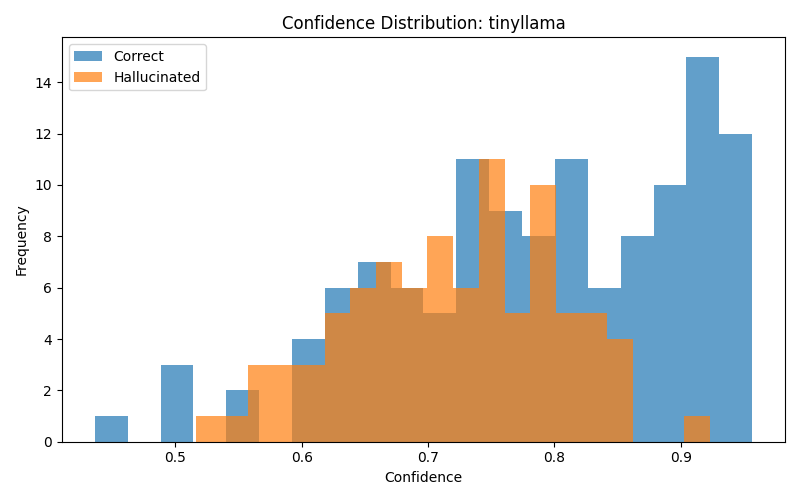
\includegraphics[width=0.45\textwidth]{images/tinyllama_confidence_histogram.png}
    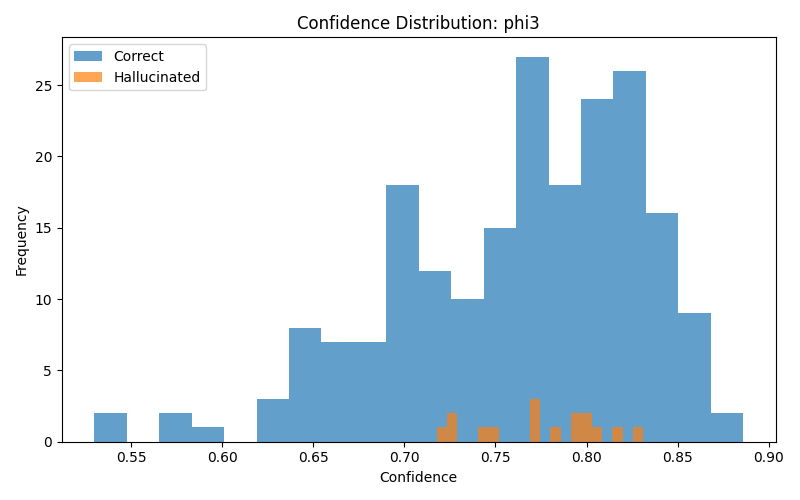
\includegraphics[width=0.45\textwidth]{images/phi3_confidence_histogram.png}
    \caption{Confidence distributions for TinyLlama and Phi-3 Mini. TinyLlama shows wider spread and instability, while Phi-3 demonstrates more consistent confidence behavior.}
    \label{fig:conf-small-models}
\end{figure}

\begin{figure}[H]
    \centering
    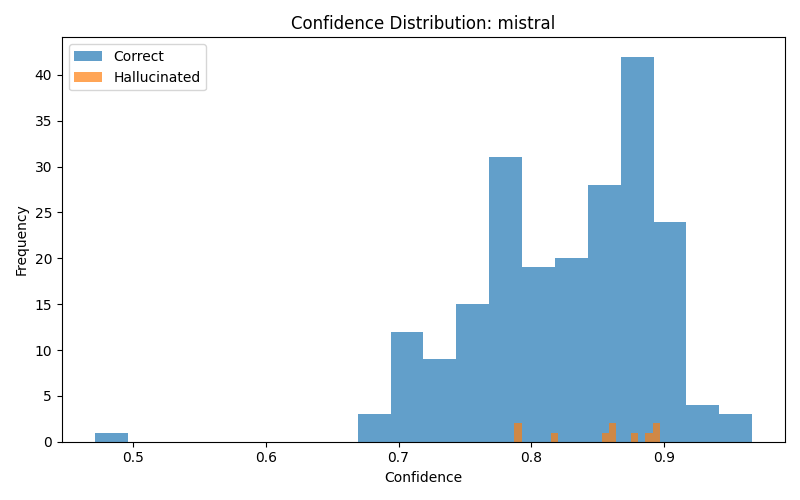
\includegraphics[width=0.45\textwidth]{images/mistral_confidence_histogram.png}
    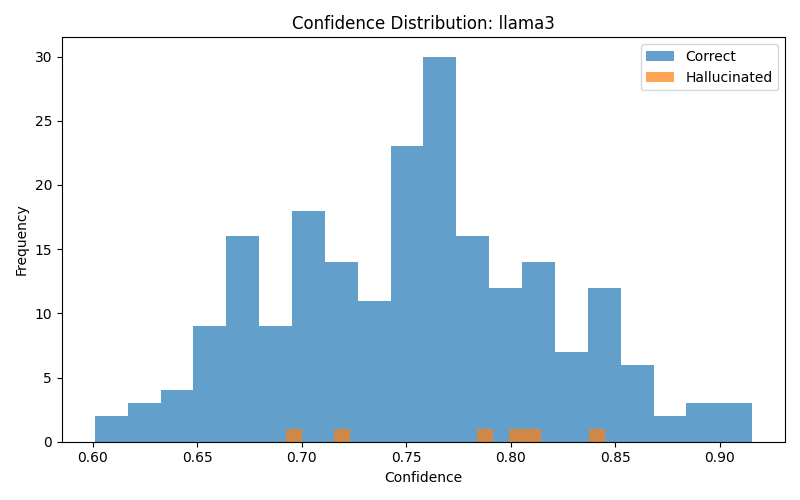
\includegraphics[width=0.45\textwidth]{images/llama3_confidence_histogram.png}
    \caption{Confidence distributions for Mistral 7B and LLaMA 3.1. Both models exhibit tighter distributions, though high confidence is still observed even in incorrect responses.}
    \label{fig:conf-large-models}
\end{figure}

+



\subsection{Labeling Strategy}
The benchmark uses a response-level labeling rule that distinguishes hallucination from safe refusal. Each generated answer is mapped into one of three functional behaviors:
\begin{enumerate}[leftmargin=1.5em]
    \item \textbf{Correct}: the answer matches the factual target, or in the case of invalid prompts, the model correctly rejects the premise.
    \item \textbf{Refusal}: the model explicitly signals that the answer cannot be determined, that the premise is false, or that the entity does not exist.
    \item \textbf{Hallucination}: the answer is incorrect \emph{and} the model does not refuse; it fabricates or plays along.
\end{enumerate}

This rule was chosen deliberately. Earlier simplistic heuristics such as ``incorrect + high confidence = hallucination'' are too narrow for a benchmark of this type, because a fabricated answer can still be harmful even when the confidence score is only moderate. By explicitly modeling refusal, the benchmark better separates uncertainty-aware behavior from fabricated outputs.

\subsection{Dataset Size}
Each of the four models was evaluated on 223 prompts, yielding a merged dataset of 892 response rows. This merged table contains question metadata, model metadata, confidence, correctness, refusal, hallucination labels, and response-length features.

\subsection{Overall Model Results}
Table~\ref{tab:model-summary} summarizes overall behavior.

\begin{table}[H]
\centering
\caption{Overall model performance on the 223-prompt benchmark.}
\label{tab:model-summary}
\begin{tabular}{lrrrrr}
\toprule
Model & Total & Accuracy & Hallucination Rate & Refusal Rate & Avg. Confidence \\
\midrule
LLaMA 3.1 & 223 & 0.9596 & 0.0269 & 0.6682 & 0.7537 \\
Mistral 7B & 223 & 0.9462 & 0.0448 & 0.6188 & 0.8273 \\
Phi-3 Mini & 223 & 0.9283 & 0.0717 & 0.5202 & 0.7628 \\
TinyLlama & 223 & 0.5561 & 0.4036 & 0.3139 & 0.7584 \\
\bottomrule
\end{tabular}
\end{table}

Several patterns stand out. First, the strongest models perform extremely well on this simple benchmark. That is expected and consistent with the benchmark's role as a demonstration dataset. Second, TinyLlama hallucinates much more often, which is useful for exposing the phenomenon more clearly. Third, refusal rates are high for the strongest models, especially in categories designed to trigger uncertainty. This suggests that refusal is acting as an important safety mechanism rather than as a weakness.

\begin{figure}[H]
    \centering
    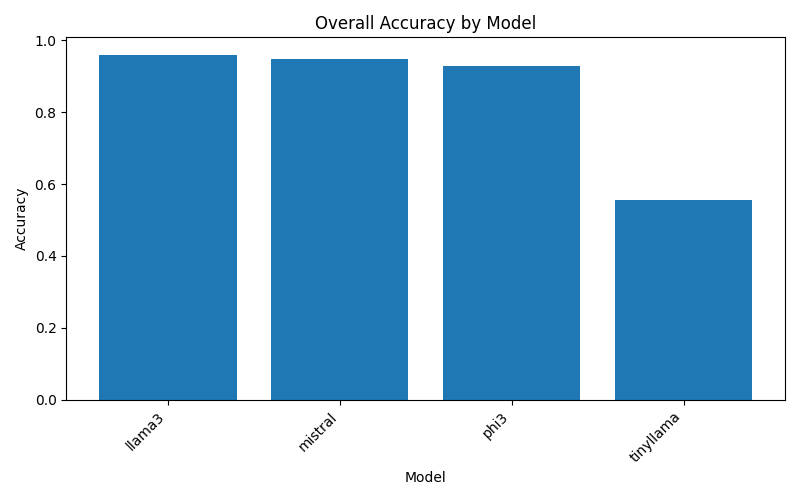
\includegraphics[width=0.75\textwidth]{images/overall_accuracy_by_model.png}
    \caption{Overall accuracy by model across the 223-prompt benchmark. Larger instruction-tuned models achieved substantially higher accuracy than TinyLlama on this demonstration-oriented dataset.}
    \label{fig:overall-accuracy}
\end{figure}

\begin{figure}[H]
    \centering
    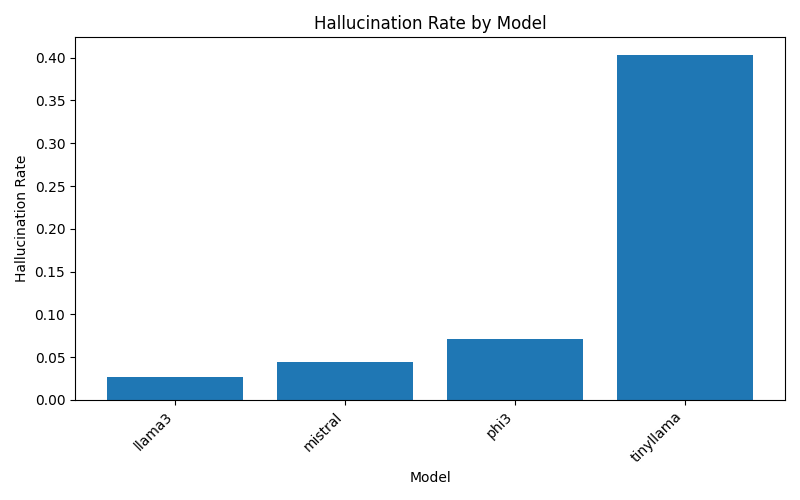
\includegraphics[width=0.75\textwidth]{images/hallucination_rate_by_model.png}
    \caption{Hallucination rate by model across the benchmark. TinyLlama produces hallucinated responses far more frequently than larger models, highlighting the impact of model scale and instruction tuning.}
    \label{fig:hallucination-rate}
\end{figure}

\begin{figure}[H]
    \centering
    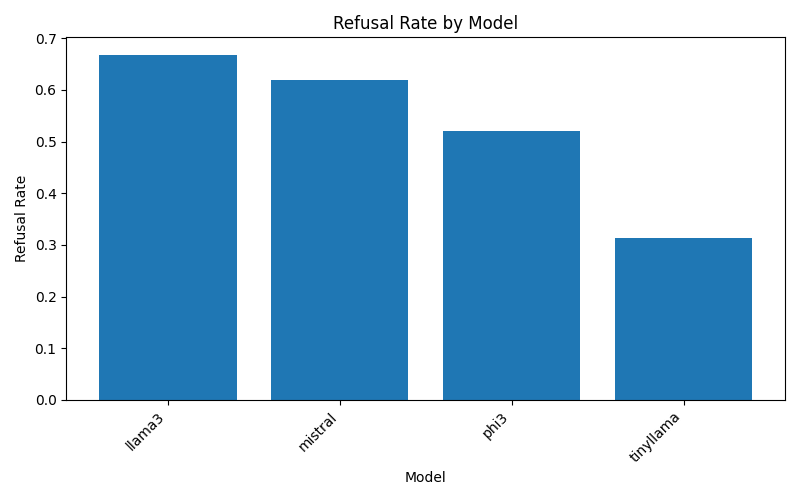
\includegraphics[width=0.75\textwidth]{images/refusal_rate_by_model.png}
    \caption{Refusal rate by model. Stronger models are more likely to refuse answering invalid or uncertain prompts, indicating that refusal behavior acts as a key safety mechanism.}
    \label{fig:refusal-rate}
\end{figure}

\newpage
\subsection{Category-Level Analysis}
Aggregating across all models yields the category-level summary in Table~\ref{tab:category-summary}.

\begin{table}[H]
\centering
\caption{Category-level performance aggregated across all four models.}
\label{tab:category-summary}
\begin{tabular}{lrrrr}
\toprule
Category & Total & Accuracy & Hallucination Rate & Refusal Rate \\
\midrule
Adversarial & 204 & 0.8039 & 0.1961 & 0.8039 \\
Easy & 236 & 0.9619 & 0.0339 & 0.2246 \\
Hard & 232 & 0.7888 & 0.1552 & 0.3190 \\
Trap & 220 & 0.8273 & 0.1727 & 0.8273 \\
\bottomrule
\end{tabular}
\end{table}

These results align with the benchmark design. Easy prompts are handled well by nearly all models, which reinforces the point that the benchmark is intentionally lightweight. Hard prompts produce more hallucination because knowledge becomes less accessible. Trap and adversarial prompts strongly increase refusal rates, especially for the stronger models, indicating that instruction tuning and alignment help models avoid confidently answering nonsense or impossible questions.

\begin{figure}[H]
    \centering
    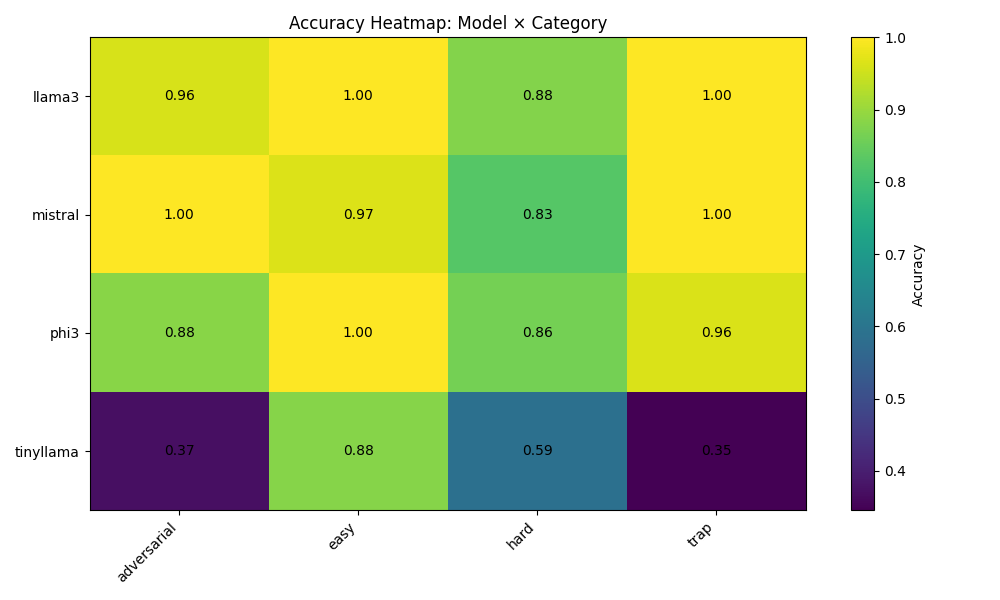
\includegraphics[width=0.85\textwidth]{images/accuracy_heatmap_model_by_category.png}
    \caption{Accuracy heatmap by model and prompt category. Easy prompts are handled reliably across models, while hard prompts reveal performance gaps, especially for smaller models.}
    \label{fig:accuracy-heatmap}
\end{figure}

\begin{figure}[H]
    \centering
    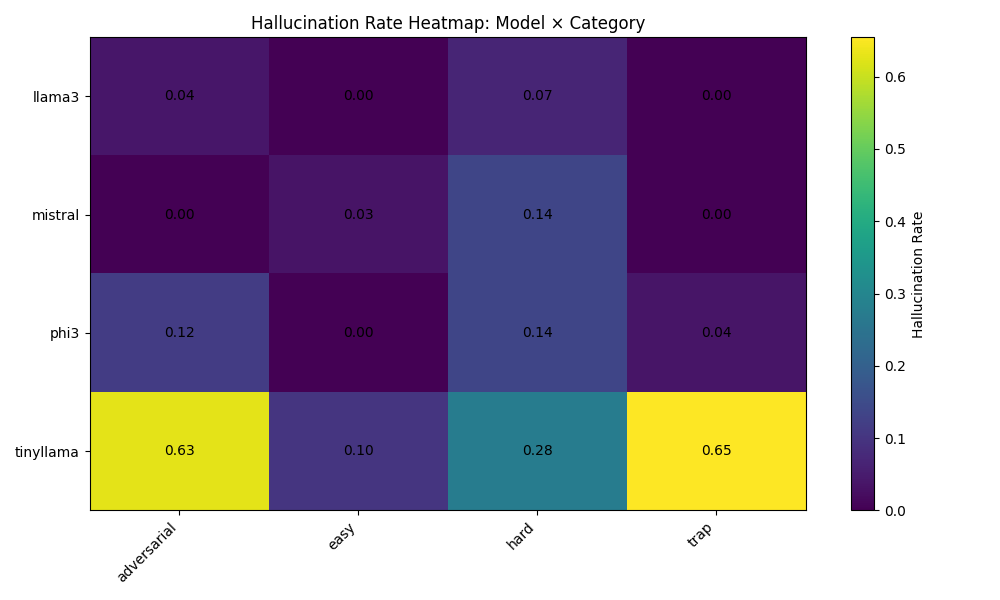
\includegraphics[width=0.85\textwidth]{images/hallucination_heatmap_model_by_category.png}
    \caption{Hallucination rate heatmap by model and category. Hallucinations are more prevalent in hard, trap, and adversarial prompts.}
    \label{fig:hallucination-heatmap}
\end{figure}

\begin{figure}[H]
    \centering
    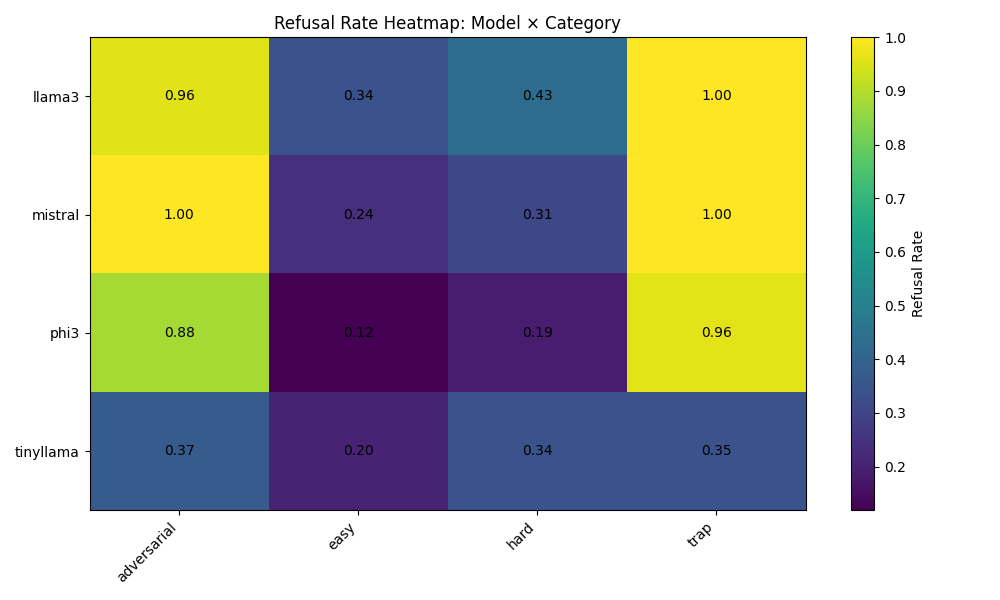
\includegraphics[width=0.85\textwidth]{images/refusal_heatmap_model_by_category.png}
    \caption{Refusal rate heatmap by model and category. Trap and adversarial prompts trigger higher refusal rates, especially in larger models.}
    \label{fig:refusal-heatmap}
\end{figure}

\newpage
\subsection{Interpreting the Low Hallucination Rates of Stronger Models}
An important interpretive point follows from these tables: the low hallucination rates of LLaMA 3.1, Mistral, and Phi-3 on this benchmark should \emph{not} be generalized to all deployments. This benchmark contains mostly straightforward prompts, simple factual questions, and intentionally constructed traps that stronger instruction-tuned systems can often reject. That does \emph{not} imply these models are safe or non-hallucinatory in domains where:
\begin{itemize}[leftmargin=1.5em]
    \item facts are long-tail or newly changing,
    \item domain expertise is needed to verify correctness,
    \item source attribution matters,
    \item unsupported confident answers can cause harm.
\end{itemize}

The broader literature strongly suggests that legal and medical contexts remain much harder. Legal studies have documented severe hallucination rates on specific case-law queries \cite{dahl2024legal}. Medical benchmarks similarly show that domain-specific hallucination remains a major unresolved problem \cite{pal2023medhalt, pandit2025medhallu}. Therefore, the strongest claim supported by the present benchmark is not that advanced models are ``safe,'' but that modern aligned models can suppress many errors on simple prompts by refusing more often.

\subsection{Confidence Versus Correctness}
The benchmark also examines whether confidence is a reliable indicator of truthfulness. The answer is no: confidence is useful, but insufficient. In the strongest models, average confidence on hallucinated answers remains relatively high. For example, LLaMA 3.1 and Mistral both show average hallucinated confidence above 0.77 and 0.85 respectively in the project outputs. This supports a familiar concern in the literature: models may be wrong while still sounding and behaving certain \cite{lin2022truthfulqa, huang2023survey}.

\begin{figure}[H]
    \centering
    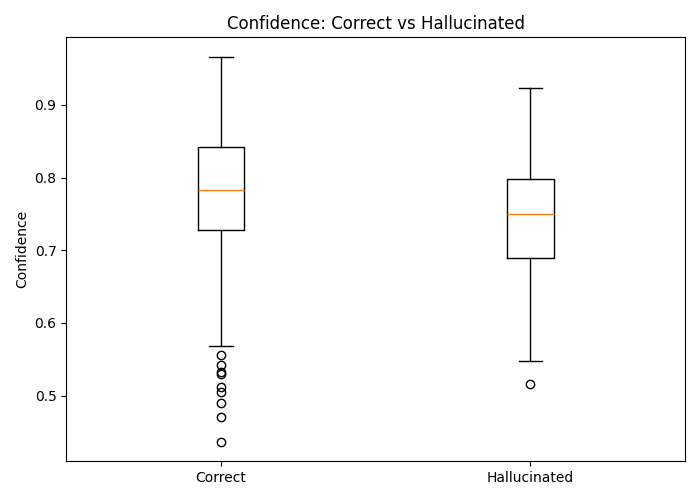
\includegraphics[width=0.75\textwidth]{images/confidence_boxplot_correct_vs_hallucinated.png}
    \caption{Confidence comparison between correct and hallucinated responses. Hallucinated responses still maintain relatively high confidence.}
    \label{fig:confidence-boxplot}
\end{figure}

\begin{figure}[H]
    \centering
    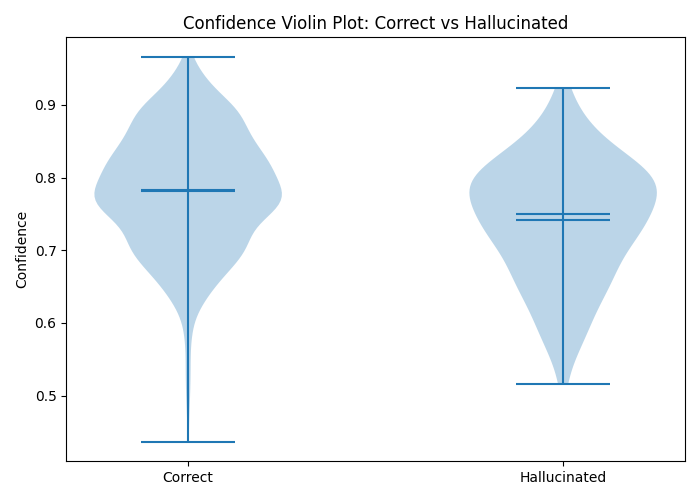
\includegraphics[width=0.75\textwidth]{images/confidence_violin_correct_vs_hallucinated.png}
    \caption{Distribution overlap between correct and hallucinated confidence values. The overlap highlights that confidence alone is insufficient for detecting hallucination.}
    \label{fig:confidence-violin}
\end{figure}

\begin{figure}[H]
    \centering
    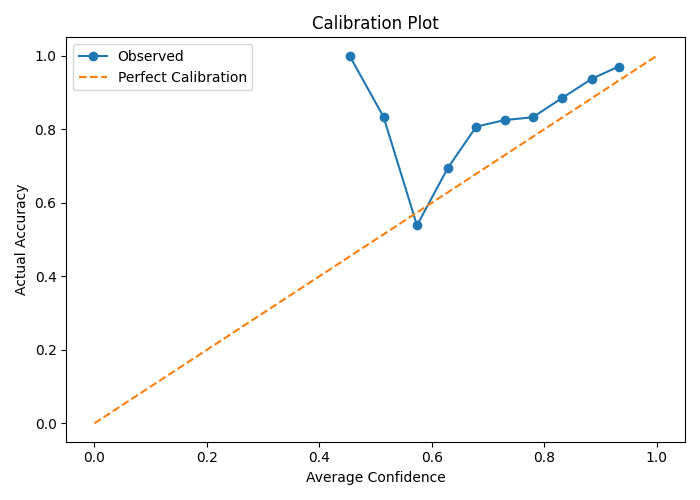
\includegraphics[width=0.75\textwidth]{images/calibration_plot.png}
    \caption{Calibration plot comparing predicted confidence against actual correctness. Deviations from the diagonal indicate imperfect confidence calibration.}
    \label{fig:calibration}
\end{figure}

\subsection{Part I Discussion}
Part I demonstrates the central problem successfully:
\begin{enumerate}[leftmargin=1.5em]
    \item small and medium open models can hallucinate substantially,
    \item stronger instruction-tuned models still hallucinate in some cases,
    \item refusal behavior is a major mechanism by which stronger models reduce observable hallucination,
    \item confidence alone is not enough to determine factual reliability.
\end{enumerate}

This part of the project therefore establishes a useful demonstration benchmark, but not a final answer to truthfulness evaluation. Its strongest value is pedagogical and diagnostic: it creates a reproducible setting in which hallucination can be observed, quantified, and used to train a downstream detector.

\newpage
\section{Part II: Response-Level Hallucination Detection with Machine Learning}

\subsection{Motivation}
Once the benchmark data are collected, a natural next question is whether hallucination can be detected automatically. The detector in this project is designed as a \emph{post-response classifier}. It does not attempt to predict whether a prompt \emph{will} cause hallucination before generation. Instead, it examines a completed response and predicts whether that response is hallucinated.

This framing matters in practice. In many applications, the system already has the generated answer in hand, so a second-stage detector can be used to flag risky outputs, trigger fallback behavior, or request additional grounding.

\subsection{Learning Problem}
The detection target is the binary hallucination label generated during Part I. The input features are tabular, drawn from the response and metadata:
\begin{itemize}[leftmargin=1.5em]
    \item confidence,
    \item question length,
    \item answer length,
    \item length ratio,
    \item confidence $\times$ answer length,
    \item low-confidence flag,
    \item refusal,
    \item category,
    \item model name,
    \item question validity.
\end{itemize}

The detector therefore learns from behavioral and structural signals rather than semantic embeddings of the full answer text. This choice keeps the modeling pipeline simple and interpretable.

\subsection{Models Trained}
Two classical models were trained:
\begin{itemize}[leftmargin=1.5em]
    \item Logistic Regression
    \item Random Forest
\end{itemize}

These models are suitable for a first-stage detector because they are fast to train, interpretable, and appropriate for structured response-level features. The train/test split uses stratification on the hallucination label to preserve class balance between train and test sets.

\subsection{Evaluation Metrics}
The detector is evaluated using:
\begin{itemize}[leftmargin=1.5em]
    \item Accuracy
    \item Precision
    \item Recall
    \item F1 score
    \item ROC-AUC
    \item Average Precision
\end{itemize}

Because the goal is to identify hallucinations, recall is especially important. Missing hallucinations corresponds to letting risky outputs pass as safe. However, precision also matters because too many false alarms would make the detector less useful operationally. The final threshold used for both models is 0.40.

\subsection{Detector Results}
Table~\ref{tab:detector-results} summarizes final detector performance.

\begin{table}[H]
\centering
\caption{Hallucination detector performance on the held-out test set.}
\label{tab:detector-results}
\begin{tabular}{lrrrrrr}
\toprule
Model & Accuracy & Precision & Recall & F1 & ROC-AUC & AP \\
\midrule
Logistic Regression & 0.8715 & 0.5122 & 0.8750 & 0.6462 & 0.9589 & 0.8545 \\
Random Forest & 0.9330 & 0.7000 & 0.8750 & 0.7778 & 0.9583 & 0.8740 \\
\bottomrule
\end{tabular}
\end{table}

The Random Forest is the stronger model overall. It matches Logistic Regression on recall, which is important because both models detect 87.5\% of hallucinations in the test set. However, it improves precision substantially, from 0.512 to 0.700, meaning it generates fewer false hallucination alarms while preserving high sensitivity.

\subsection{Confusion Matrix Interpretation}
The held-out test set contains 179 responses, with 24 positive hallucination examples and 155 non-hallucination examples. From the reported precision, recall, and support values, the confusion matrices can be reconstructed.

\paragraph{Logistic Regression.}
\begin{center}
TN = 135, \quad FP = 20, \quad FN = 3, \quad TP = 21
\end{center}

\begin{figure}[H]
    \centering
    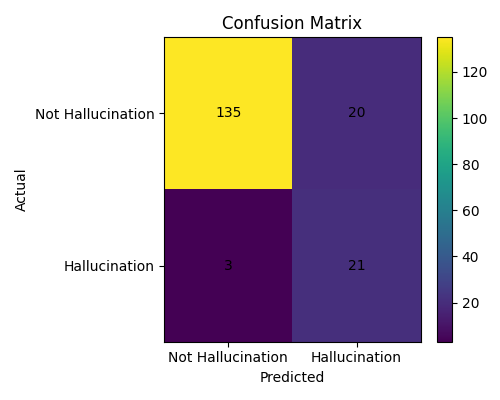
\includegraphics[width=0.61\textwidth]{images/logistic_regression_confusion_matrix.png}
    \caption{Confusion matrix for Logistic Regression detector. High recall but more false positives compared to Random Forest.}
    \label{fig:logreg-cm}
\end{figure}

\paragraph{Random Forest.}
\begin{center}
TN = 146, \quad FP = 9, \quad FN = 3, \quad TP = 21
\end{center}

\begin{figure}[H]
    \centering
    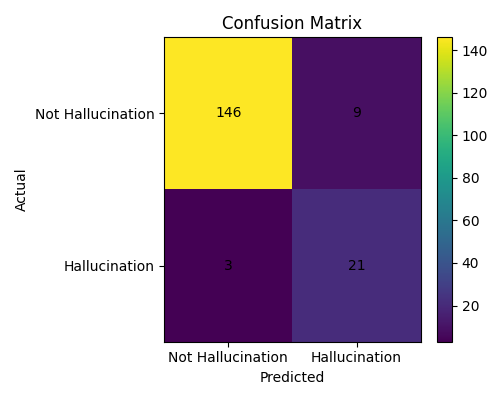
\includegraphics[width=0.61\textwidth]{images/random_forest_confusion_matrix.png}
    \caption{Confusion matrix for Random Forest detector. Improved balance with fewer false positives while maintaining high recall.}
    \label{fig:rf-cm}
\end{figure}

The key improvement is that the Random Forest reduces false positives from 20 to 9 while preserving the same number of true positives and false negatives. That is a meaningful improvement for a practical second-stage detector.

\paragraph{Figure placeholder.}
\texttt{<include reports/plots/detector/logistic\_regression\_confusion\_matrix.png here>}

\paragraph{Figure placeholder.}
\texttt{<include reports/plots/detector/random\_forest\_confusion\_matrix.png here>}

\subsection{ROC and Precision--Recall Interpretation}
Both models achieve ROC-AUC around 0.958, which indicates excellent ranking performance. In other words, even when thresholding changes, the models are generally able to assign higher risk scores to hallucinated answers than to non-hallucinated ones.

Precision--Recall analysis is also strong, with the Random Forest achieving average precision of 0.874. This is important because hallucination detection is often class-imbalanced in real datasets: correct or safely refused answers may be more common than hallucinations. In those settings, Average Precision can be more informative than ROC-AUC alone.

\begin{figure}[H]
    \centering
    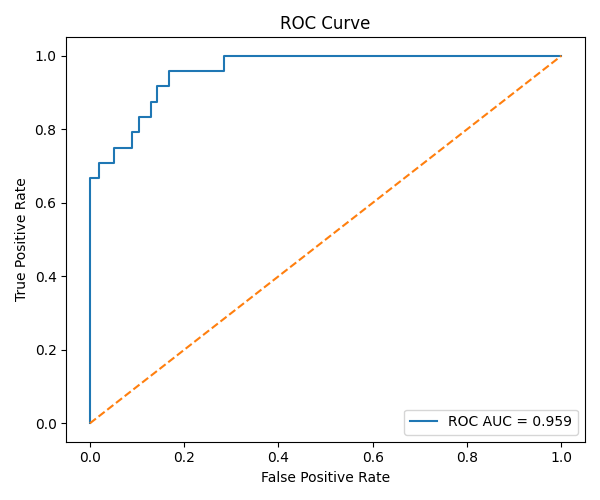
\includegraphics[width=0.7\textwidth]{images/logistic_regression_roc_curve.png}
    \caption{ROC curve for Logistic Regression. Demonstrates strong classification capability across thresholds.}
    \label{fig:logreg-roc}
\end{figure}

\begin{figure}[H]
    \centering
    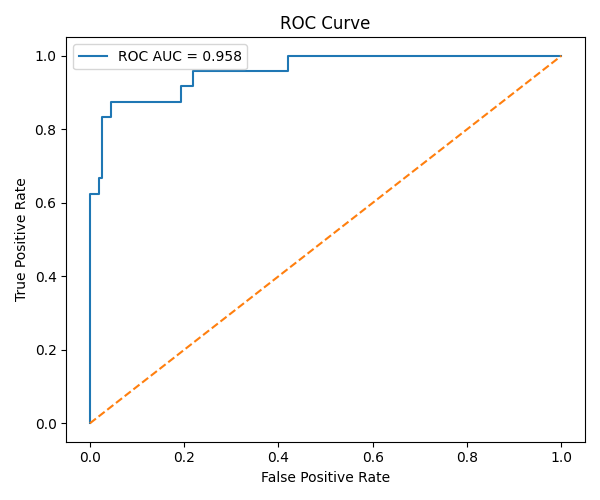
\includegraphics[width=0.7\textwidth]{images/random_forest_roc_curve.png}
    \caption{ROC curve for Random Forest detector. Shows excellent separability between hallucinated and non-hallucinated responses.}
    \label{fig:rf-roc}
\end{figure}

\begin{figure}[H]
    \centering
    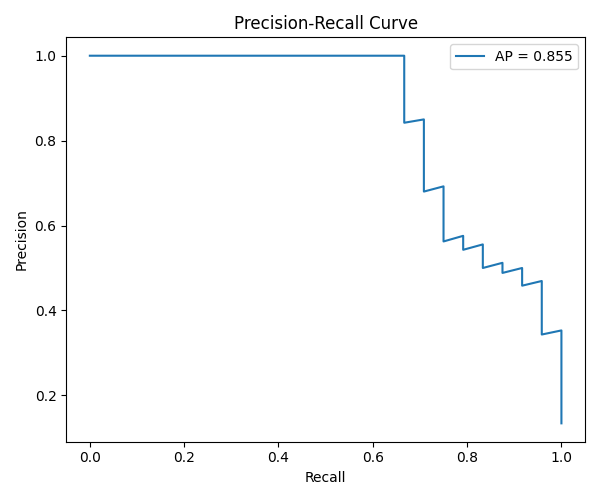
\includegraphics[width=0.7\textwidth]{images/logistic_regression_pr_curve.png}
    \caption{Precision-Recall curve for Logistic Regression. Highlights strong recall but moderate precision.}
    \label{fig:logreg-pr}
\end{figure}

\begin{figure}[H]
    \centering
    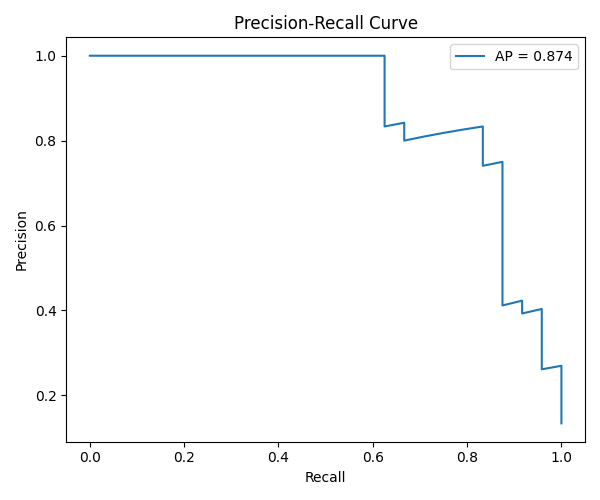
\includegraphics[width=0.7\textwidth]{images/random_forest_pr_curve.png}
    \caption{Precision-Recall curve for Random Forest. Demonstrates better precision-recall tradeoff.}
    \label{fig:rf-pr}
\end{figure}

\subsection{Feature Importance and What the Detector Learns}
The Random Forest feature-importance plot indicates that refusal behavior is the dominant signal, followed by model identity, confidence, answer length interactions, and prompt category. This is a meaningful result. It suggests that the detector is not simply learning ``low confidence equals hallucination.'' Instead, it learns a richer behavioral rule:
\begin{quote}
hallucinated answers tend to be \emph{wrong and non-refusing}, while safer model behavior is strongly associated with explicit refusal or premise rejection.
\end{quote}

This aligns closely with the benchmark design and with the qualitative behavior seen in strong instruction-tuned systems. Refusal is not merely an artifact in this project; it emerges as a central protective behavior. The importance of refusal also resonates with recent literature emphasizing that uncertainty-aware behavior and ``not sure'' options can improve safety-critical detection settings \cite{pandit2025medhallu}.

\begin{figure}[H]
    \centering
    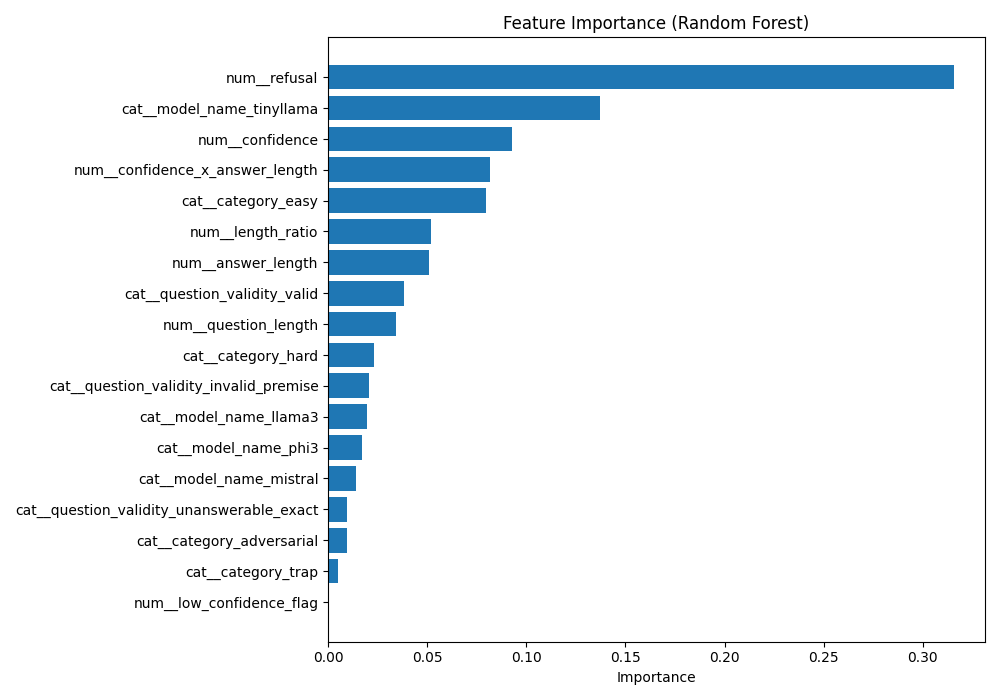
\includegraphics[width=0.8\textwidth]{images/random_forest_feature_importance.png}
    \caption{Feature importance for Random Forest detector. Refusal emerges as the most influential feature, followed by confidence and contextual features.}
    \label{fig:rf-importance}
\end{figure}

\subsection{What the Detector Actually Detects}
It is important to describe the detector precisely. This model does \emph{not} predict whether a prompt itself is dangerous before generation. It predicts whether a \emph{generated response} is hallucinated after the model has already answered. Thus the detector's role is:
\begin{center}
Prompt $\rightarrow$ LLM Answer $\rightarrow$ Detector $\rightarrow$ Hallucination / Not Hallucination
\end{center}

This framing makes the detector directly useful for post-generation quality control, fallback routing, or safety warnings. It is also why response-level features such as refusal and answer length are informative.

\subsection{Part II Discussion}
Part II shows that even a relatively simple, classical ML pipeline can perform strongly when trained on a well-labeled response dataset. The Random Forest results indicate that hallucination is not a random failure mode from the detector's perspective. Instead, hallucinated responses exhibit learnable structure:
\begin{itemize}[leftmargin=1.5em]
    \item they are less likely to include refusal signals,
    \item they often appear with nontrivial confidence,
    \item they depend on model identity and prompt category,
    \item they can be distinguished from non-hallucinated outputs with high recall.
\end{itemize}

At the same time, the detector inherits the limitations of the underlying benchmark. Because the benchmark itself is simple and domain-light, the detector is best interpreted as a proof of concept. It should not be assumed to generalize out of the box to legal, medical, or political QA without domain-specific data and stronger semantic evaluation.

\section{Threats to Validity and Limitations}
Several limitations should be stated clearly.

\subsection{Benchmark Simplicity}
The benchmark is deliberately simple. This is a feature for demonstration, but a limitation for external validity. Advanced models may appear highly reliable because many prompts are within their well-covered knowledge distribution.

\subsection{No Domain-Expert Verification in High-Stakes Fields}
The project intentionally avoids claiming results in domains such as law or medicine because the author did not build an expert-verified benchmark in those areas. This is a responsible constraint. The literature shows that hallucination rates can remain high in such domains even for strong models \cite{dahl2024legal, pal2023medhalt, pandit2025medhallu}.

\subsection{Confidence Is a Proxy, Not Ground Truth}
The confidence signal is based on average token probabilities. That measure can be informative but is not a calibrated truth score. Models can be wrong while assigning high next-token probability to their own continuation.

\subsection{Labeling Heuristics}
Although the refusal-aware labeling rule is stronger than a pure confidence threshold, it is still heuristic in the sense that correctness is resolved using a structured benchmark rather than a full semantic adjudication system. In broader settings, richer equivalence checking or expert annotation would be beneficial.

\subsection{Detector Generalization}
The detector is trained only on outputs from the four selected models and on the collected prompt distribution. Its performance should therefore be interpreted as within-distribution performance, not as universal hallucination detection.

\section{Implications}
Despite these limitations, the project supports several important conclusions.

First, hallucination remains a visible and measurable problem even on relatively simple benchmark setups. Second, refusal is one of the clearest behavioral differentiators between safer and riskier model outputs. Third, response-level detection is feasible: one does not need a giant neural detector to obtain strong results on structured benchmark data. Fourth, benchmark simplicity can mask the real difficulty of truthfulness evaluation. A model that looks strong on basic factual prompts may still be unsafe in domains that require expert grounding.

These points support a broader practical recommendation: any real deployment that relies on LLMs for factual tasks should combine generation with external evidence, verification, or retrieval support rather than assuming that apparent fluency or internal confidence is enough \cite{bechard2024rag, zhang2025ragreview}.

\newpage
\section{Conclusion}
This report presented a two-part research project on hallucination in modern LLMs. Part I constructed a demonstration benchmark and showed how hallucination, refusal, and confidence behavior differ across four instruction-tuned models. The strongest models produced relatively low hallucination rates on this simple benchmark, but that result should be interpreted cautiously: it reflects the benchmark's intentionally modest difficulty, not the absence of hallucination risk in general.

Part II trained a response-level hallucination detector on the collected dataset. A Random Forest classifier achieved strong held-out performance, showing that hallucinated outputs are behaviorally and structurally distinguishable from correct or safely refused outputs. The most important signal was refusal behavior, suggesting that one of the clearest markers of safer model behavior is the ability to say, in effect, ``I do not know,'' ``this premise is false,'' or ``this cannot be answered as asked.''

The central contribution of the project is therefore methodological and educational: it demonstrates how hallucination can be measured, how labeling strategy changes the interpretation of model behavior, and how even a lightweight benchmark can support a useful second-stage detector. The central caution is equally important: because advanced LLMs may look reliable on simple prompts while still hallucinating in specialized settings, trustworthy deployment ultimately requires stronger grounding, richer
benchmarks, and domain-aware verification.

\section{Source Code}

The full implementation, dataset, and experimental pipeline are publicly available at
\href{https://github.com/twok-teks/llm-hallucination-analysis}{GitHub Repo}.

\newpage
\bibliographystyle{plain}
\bibliography{hallucination_refs}

\end{document}